\chapter{Preliminary Studies}
\label{Preliminary Studies}
\lhead{Chapter 5. \emph{Preliminary Studies}}

This chapter examines the development methodologies in section \ref{section:development-methodology}
and some of our earlier experiences in section \ref{section:earlier-experience}.
Section \ref{section:existing-solutions} covers already exiting solutions.
Section \ref{section:used-technologies} describes the technologies used in the project.
Testing methodologies are described in section \ref{section:testing}.
We draw our conclusions in section \ref{section:summary}.

%-----------
% SECTION 1
%-----------

\section{Development Methodology}
\label{section:development-methodology}

In this section we are going to present and discuss two common development methodologies.
We are going to conclude with what type of development methodology we chose and why we chose it.
This was one of the first discussions we had before starting the project, since without a good development process a project is often doomed to failure.
It is important to divide the work into task and work in a structured manner, in this way we will have a better understanding of where the project is and where it is headed.

%-----------------------------------
%	SUBSECTION 1
%-----------------------------------
\subsection{Waterfall Model} \nocite{WaterfallModel}

The waterfall model is a software development process where each task is performed in a sequential order.
Before moving to the next phase the preceding task needs to be finished.
The progress of the project is seen as flowing downwards through the different phases, hence the name waterfall.
This is represented in figure \ref{figure:waterfall-model} where it is possible to see how the progress is flowing.
In the original model the phases consisted of seven different tasks:

\begin{enumerate}
\item Requirements specification
\item Design
\item Construction (implementation or coding)
\item Integration
\item Testing and debugging
\item Installation
\item Maintenance
\end{enumerate}

\begin{figure}[h]
\begin{center}
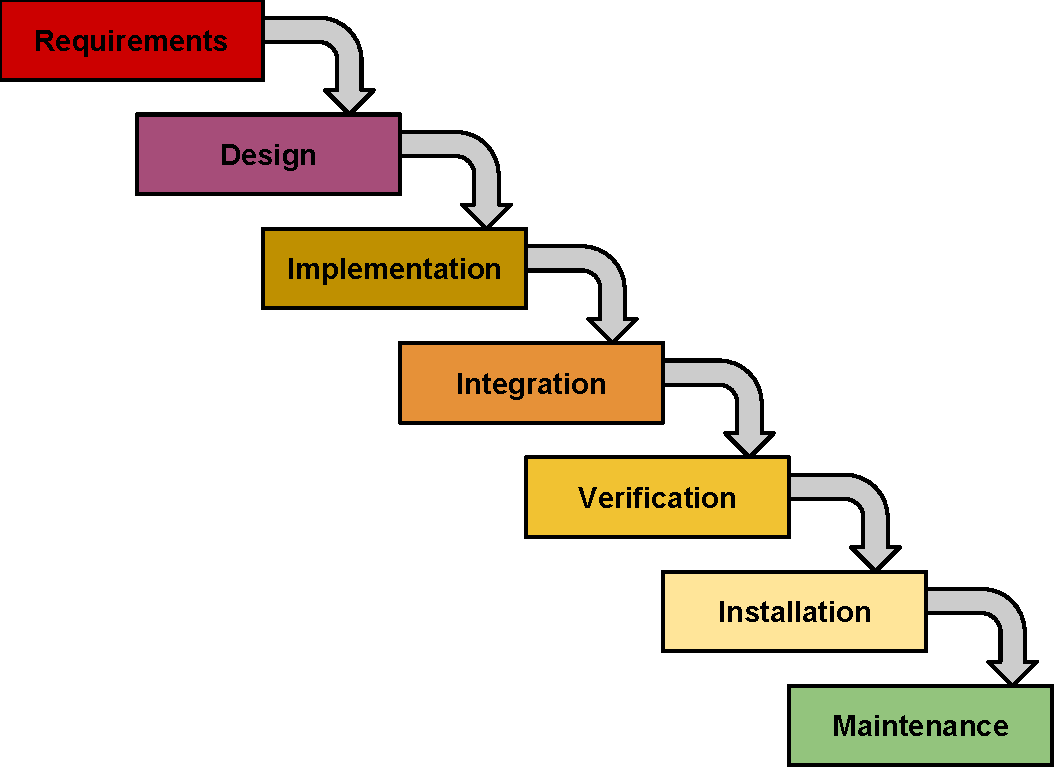
\includegraphics[scale=0.6]{../Figures/Waterfall-model.pdf}
\end{center}
\caption{Waterfall model}
\label{figure:waterfall-model}
\end{figure}

Because each phase needs to be perfected and completed before moving to the next phase, it will bring up some difficulties if the requirements were to change during the development process. 
However, the model is easily understandable, structured, and disciplined. 
All the phases are divided into different sections, and this makes it easier to understand the progress of the project.
In practice it can be very hard to adapt to this kind of development model. 
It can be hard for a system designer to predict future implementation difficulties of a type of design, hence the design of the system may change during the process.
Another problem is that the customer is not always sure about the system requirements, and will often change them during the development.

%-----------------------------------
%	SUBSECTION 2
%-----------------------------------
\subsection{Scrum Model} \nocite{Compendium}
%cite http://www.mountaingoatsoftware.com/agile/scrum

Scrum is an emerging agile development process which is mostly used in software development.
The Scrum approach, which could be described as both iterative and incremental, consists of multiple sprints
which last from two to four weeks. Sprints begin with a planning meeting and conclude with a review meetings.

During this meeting team members produce a \emph{sprint backlog}: an artifact which defines a set of concrete goals
of the sprint and can be seen basically as a \''to-do\'' list of the tasks to be performed.

Such tasks, which in Scrum's terminology are called \emph{stories} are taken from the
\emph{product backlog} which is a prioritized list of the requirements of the product.

Although a product backlog is usually made during the early stages of the project, it is subject to
change in order to accomodate new or modified requirements.

The person in charge of populating the product backlog is called \emph{product owner}.

Each day in a sprint should begin with a meeting called \emph{daily scrum}.

During this meeting which lasts usually fifteen minutes, everybody shares the work
accomplished since the last daily meeting and their plan for the day, mentioning eventual
problems if any.
%For each day a daily scrum meeting should be performed.
%Each sprint is focusing on a set of concrete goals that are in the sprint backlog.
%The sprint backlog consists of tasks that are chosen from the product backlog. 
%They are usually chosen in the sprint planning meeting that is performed before each sprint.
%The product backlog consists of all the features the product should contain, and is usually made in the initial phase of the project.
%It can however be changed and adjusted during the development of the product.

 
Usually a scrum meeting consists of getting to know what each person did yesterday, what they will do today and if they are facing any problems.
If there are any problems the Scrum master is responsible to resolve the problem.
After each sprint a sprint review meeting should be held.
An overview of what goals where achieved and which one where not should be made.
The meeting can also consist of a demo of the new features implemented. 
Figure \ref{figure:scrum-workflow} shows the workflow of scrum.

\begin{figure}[h]
\begin{center}
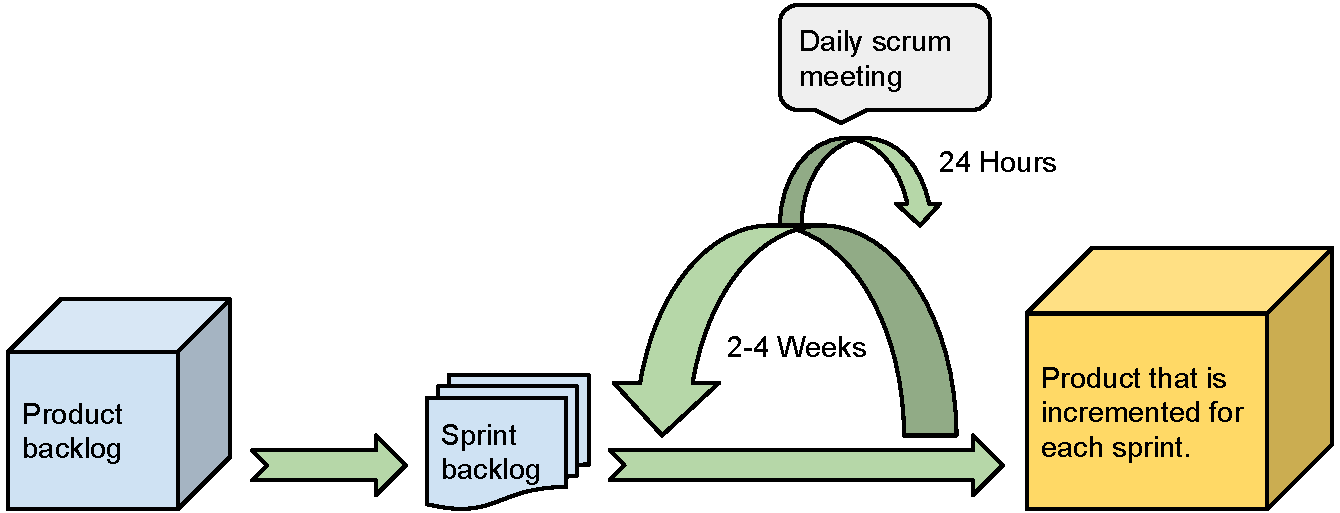
\includegraphics[scale=0.5]{../Figures/Scrum-workflow.pdf}
\end{center}
\caption{Scrum workflow}
\label{figure:scrum-workflow}
\end{figure}

%-----------------------------------
%	SUBSECTION 3
%-----------------------------------
\subsection{Conclusion}

We decided to choose the scrum model as our development process. 
The reason for this is that we didn't have a formal requirement list of the project from the beginning.
Thus it was a high probability that we didn't understand the problem completely, and might have done some wrong design decisions in the first phase of the project. 
With the Scrum method it is also a lot easier to adjust the project direction if we are going down the wrong path.
Our customer also advised us to use an agile method as our development methodology.
We thought that scrum would be a good methodology as it is a widely known and respected development process in the programming community.
The ability to change the design and choices we had made earlier in the project was very important to us.
If we for example were to make a choice that the customer wasn't pleased with, we would have the ability to fix the problem in the next sprint.
This would have been very hard to do in a non agile development methodology like the waterfall model.

%----------------------------------------------------------------------------------------
%	SECTION 2
%----------------------------------------------------------------------------------------

\section{Earlier Experience}
\label{section:earlier-experience}

This section contains a short description of our earlier experiences.
In the conclusion we give some short details of what kind of effect this had on our project.

%-----------------------------------
%	SUBSECTION 1
%-----------------------------------
\subsection{Competencies}

One of the first things we did during our first meetings was to get to know each others experiences and competencies.
This was important for us, so we could decide what type of technologies to use in our project.
In table \ref{table:competencies} we have listed our competencies in the different languages and frameworks.
We gave each technology a score from 1 to 5, where 5 indicated that the language or framework was well known and 1 indicated that it was not known.

\begin{table}
\begin{center}
\begin{tabular}{ l | l | l | l }
  \hline
  & Emanuele & Anders & Sebastian \\ \hline
  HTML & 4 & 4 & 4 \\
  CSS  & 1 & 4 & 4 \\
  JavaScript & 2 & 4 & 5 \\
  Java & 5 & 5 & 5 \\
  Maven & 2 & 3 & 1 \\
  Angular & 1 & 2 & 1 \\
  Git & 4 & 5 & 4 \\
  NodeJS & 1 & 1 & 1 \\
  jQuery & 1 & 1 & 4 \\
  SQL & 3 & 4 & 4 \\
  Spring & 1 & 3 & 1 \\
  \hline
\end{tabular}
\end{center}
\caption{Competencies}
\label{table:competencies}
\end{table}

%-----------------------------------
%	SUBSECTION 2
%-----------------------------------
\subsection{Conclusion}

We managed to find out our competencies, and fortunately many of us already had the experience that was needed to start a project like this.
This was of great help to us when deciding what technologies to use in our project.
In table \ref{table:competencies} it is also visible that some of us were more familiar with some technologies than other.
This made it easier to divide the tasks between each other in the project.

%----------------------------------------------------------------------------------------
%	SECTION 3
%----------------------------------------------------------------------------------------

\section{Existing Solutions}
\label{section:existing-solutions}

This section describes similar existing solutions.
The following technologies were a good inspiration source and help in our project,
as they already were similar or did contain components that our application also would contain.

%-----------------------------------
%	SUBSECTION 1
%-----------------------------------
\subsection{HealthVault} \nocite{HealthVault}
%http://msdn.microsoft.com/en-us/healthvault/jj128027

HealthVault is Microsoft's online service to collect, store and monitor personal health information.

%and share it with other people which could family doctors or relatives.

Health records can be collected from different sources such as:
\begin{itemize}
\item smartphone or desktop applications
\item devices like step counters, blood glucose meters, weighting scales\ldots
\item third-party health services like Withings, \ldots
\end{itemize}
using the web-based XML API exposed by HealthVault.

In order to connect to HealthVault these sources need to be authorized by the user upon first use.
Health records can then be shared with other people like family members or doctors, as well as
healthcare providers. Access to stored data can be selective meaning that a source can be authorized to access a specific record (weight measurements, glucose \ldots) but not others (allergies, pregnancies\ldots).



%Technically speaking, HealthVault is in fact an XML-over-HTTP webservice.


% that can be used by developers to connect and interact
%with HealtVault.

In HealthVault a single data measurement is called a \textit{thing}.
Basically, a \textit{thing} represents a measurement of some health parameter
which could be weight or heart rate for example.

See below an XML sample of a weight \textit{thing}.
\begin{lstlisting}[language=XML]
<weight>
  <value>
    <kg>60</kg>
    <display units="kg">132</display>
  </value>
  <when>
    <date>
      <y>1990</y>
      <m>1</m>
      <d>1</d>
    </date>
    <time>
      <h>1</h>
      <m>0</m>
      <s>0</s>
    </time>
  </when>
</weight>
\end{lstlisting}

Several software development kits (SDK) are available for major mobile platforms
such as iOS, Windows Phone and Android. Additionally a number of SDKs in various
languages (Ruby, PHP, Java)
%Access to stored data can be selective meaning that a source can be authorized to access
%a specific record (weight, \ldots) but not others (glucose, \ldots).



%Additionally it is possible to store and retrieve medical images in \textit{DICOM} format.

%The devices might be weighting scales, step counters, blood glucose monitors and more.
%While the applications can be different types of mobile, tablet or desktop apps.
%It is also possible to share the information stored in HealthVault with e.g. family members or a doctor.
%It's possibile to selectively share health information with other
%people which could be family doctors or relatives.

Additionally, HealthVault supports exporting of data in industry-standard formats.
%An HealthVault account can be linked to multiple individuals.



%-----------------------------------
%	SUBSECTION 2
%-----------------------------------
\subsection{Open eHealth Foundation} \nocite{OpenEHealthFoundation}

The goal of Open eHealth Foundation is to create and share open source software components for the healthcare ICT industry.
One of their products is an integration platform called Open eHealth Integration Platform (IPF).
It is based on Apache Camel and has support for connecting systems in the eHealth domain.

%-----------------------------------
%	SUBSECTION 3
%-----------------------------------
\subsection{human/api} \nocite{HumanAPI}

The human API is a platform for human health data. 
They have an API that contains multiple different well defined JSON strings for different kinds of human related data.
Each JSON string contains all the necessary information that is needed to represent each type of health data.
For example heart rate is defined by an id, user id, time, value and unit in the following way:

\begin{verbatim}
{
  "id": "string",
  "userId": "string",
  "time": "date",
  "value": "int",
  "unit": "string"
}
\end{verbatim}

%-----------------------------------
%	SUBSECTION 4
%-----------------------------------
\subsection{Android heart rate monitor} \nocite{AndroidHeartRateMonitor}
\label{subsec: AndroidHeartRateMonitor}

Android heart rate monitor is an open source heart rate measurer for android.
It measures the heart rate of the user with help of the camera and flash light on the phone.

%-----------------------------------
%	SUBSECTION 5
%-----------------------------------
\subsection{Conclusion}

The applications mentioned above were of great help for us in our project.
Our integration platform needs to send and receive information. 
With help of the Human API we found out how the structure of this information should be.
The android application mentioned in \ref{subsec: AndroidHeartRateMonitor} was a good starting point for creating the heart rate application that we needed in our project.


%----------------------------------------------------------------------------------------
%	SECTION 4
%----------------------------------------------------------------------------------------
\section{Used Technologies}
\label{section:used-technologies}

This section contains the technologies we used in our project.
We are going to go through what type of technologies we used for the server (back-end), web page (front-end), database and for the development of applications for mobile units. 
It also contains some other technologies that were needed in the project.

%-----------------------------------
%	SUBSECTION 1
%-----------------------------------
\subsection{Server}

\textbf{Java} \nocite{Java}

Java is a general-purpose programming language, which means that it can be used in a wide variety of application domains.
It is platform independent, and thus makes it easy to develop software for different operation systems.
Web programming is one of the domains that Java is used for, hence makes it possible to write a service that runs in the back-end of a website.
The web services created with Java allows creating a bridge between the database and the front-end. 
This makes it possible to create a communication between the user and the database at the server.

\textbf{Spring Framework} \nocite{SpringFramework1}\nocite{SpringFramework2}

The Spring Framework is an open source application framework and inversion of controll container for Java. 
We use the Spring framework to set up a RESTful service and to handle the data access from the database. 

\textbf{Apache Tomcat} \nocite{ApacheTomcat}

Apache Tomcat is an implementation of the JSP (JavaServer Pages) and Java Servlet technologies.
It makes it possible to deploy and run a website with its services on a server.
Numerous industries and organizations use the Tomcat server as it has support for large-scale and mission-critical web applications.

%-----------------------------------
%	SUBSECTION 2
%-----------------------------------
\subsection{Database}

\textbf{MySQL} \nocite{MySQL}

MySQL is one of the most widely used relational database management system.
The MySQL Community Edition is open source and freely available.
It is developed to handle large databases, support many users at the same time and it is also scalable.
It makes it possible to store and retrieve data in an efficient and structured manner.

\textbf{MySQL Workbench}

MySQL Workbench is a free-to-use tool which allows to easily manage MySQL databases.
We used MySQL Workbench for database design and deployment both locally (for testing) and remotely (production).


%-----------------------------------
%	SUBSECTION 3
%-----------------------------------
\subsection{Website}

\textbf{HTML5} \nocite{HTML5}

HTML is the standard World Wide Web's markup language, where HTML5 is the newest HTML version as of this writing.
It is used to structure and visualize web pages on the internet.
By writing a document with HTML a web browser is later on able to interpret the document and visualize it in a structured manner.

\textbf{CSS3} \nocite{CSS3}

CSS describes the look and format of a document written in HTML.
It allows one to use different fonts, colors and adjust the layout of a web page.
By using CSS and separating it from the HTML, it is possible to allow multiple pages share the same style.
Thus it is easier to maintain and adapt the web pages to different environments through CSS.

\textbf{Bootstrap} \nocite{Bootstrap}

Bootstrap contains HTML and CSS templates for web designers.
This makes it easier to make a good looking web page without putting too much effort into the design.

\textbf{JavaScript} \nocite{JavaScript}

JavaScript is an interpreted computer programming language that runs in the browser of the user.
It is allowed to make changes in the HTML DOM, interact with the user, control the browser and communicate asynchronously.
Since it can communicate with the server asynchronously, it makes the web page more dynamic.
What this means is that a web page can acquire new information and change the site without reloading.

\textbf{jQuery} \nocite{jQuery}

jQuery is a JavaScript library for manipulating and traversing the HTML DOM.
All the features jQuery contains are also possible to do with pure JavaScript, but jQuery helps the developer to implement the different features in an easier way.
For example it contains predefined methods for event handling and animation.
It also makes it easier to communicate with the server through AJAX.

\textbf{Chart.js} \nocite{Chartjs}

Chart.js is a JavaScript library for creating graphs and charts.
It helps the developer to visualize data through different types of graphs in an easy manner.
The library has support for different types of two dimensional data, e.g. value per time.
It also has the ability to display multiple graphs in the same chart.

%-----------------------------------
%	SUBSECTION 4
%-----------------------------------
\subsection{Mobile Technologies}

\textbf{Android SDK} \nocite{AndroidSDK}

Android SDK contains the tools necessary for developing, debugging and testing an Android app.
With the SDK it is possible to write and modify applications for an Android phone.

%-----------------------------------
%	SUBSECTION 5
%-----------------------------------
\subsection{Other Technologies}

\textbf{Maven} \nocite{Maven}

Maven is a software tool for managing a programming project.
It has the ability to build and compile programming code based on the content of a POM (Project Object Model) file.
It keeps track of all the frameworks used, and is able to download them before building the project.

\textbf{Git} \nocite{Git}

Git is a version control system that is free and open source.
This is an important tool to keep track of all the changes made to the source code, it also makes it easier for multiple developers to work on the same source.
Git makes it easy to roll back changes made to the code, in case something was wrongly implemented.
It also has the possibility to divide the project into different branches.
Which means that the code can be copied into multiple different places, and developed separately in cases where trying out different solutions is necessary.
If a good solution is made, the branch can later on be merged together with the main branch.
It is also possible to have a branch for release versions and a development branch.

%-----------------------------------
%	SUBSECTION 6
%-----------------------------------
\subsection{Conclusion}

We chose the technologies specified above based on our earlier experience and what we found most appropriate for our solution.
Before we started this project we discussed our competencies.
This was of great help in choosing the right technologies that were going to be used.
Most of us already had some different degree of experience in most of the technologies mentioned above.
This made it much easier for us to chose the right set of frameworks and languages to work with.
For example from table \ref{table:competencies} we can see that all of us were very familiar with Java, Git and SQL.
This made it clear for us to use those technologies.

%----------------------------------------------------------------------------------------
%	SECTION 5
%----------------------------------------------------------------------------------------
\section{Testing}
\label{section:testing}

In this section we are going to go through some of the testing frameworks used in our project.

%-----------------------------------
%	SUBSECTION 1
%-----------------------------------
\subsection{JUnit} \nocite{JUnit}

JUnit is a Java framework for writing tests. It is also a good tool when using test driven development.
With help of this framework it is possible to write tests for different parts of the code, then check if it runs as it should.
It is also possible to use JUnit with Maven.
When doing so it will first run all the tests, and if the tests are successful the application will be executed.

%-----------------------------------
%	SUBSECTION 2
%-----------------------------------
\subsection{Jasmine} \nocite{Jasmine}

Jasmine is a framework for testing JavaScript code.	
It doesn't require a DOM and is also not dependent on any other frameworks.

%-----------------------------------
%	SUBSECTION 3
%-----------------------------------
\subsection{Conclusion}

When using test driven development it is important to have some frameworks for testing the code.
New bugs are often introduced to applications when extending it with new functions and features.
With help of the technologies mentioned above it is much easier to find the new bugs, and hence fix them quicker.

%----------------------------------------------------------------------------------------
%	SECTION 6
%----------------------------------------------------------------------------------------

\section{Summary}
\label{section:summary}

In this chapter we had a discussion of two common development methodologies.
We also found out that the scrum model was the best development process for our project.
Our earlier experience was described in table \ref{table:competencies}.
We also discussed some of the earlier existing solutions that were already created.
A description of each technology that was used in this project was given. 
At the end of the chapter we gave a description of some of the testing methods used.